\documentclass[../body.tex]{subfiles}
\begin{document}
Будем использовать параметр релаксации $\tau=1$ в методе Ньютона.
 \subsection{Проверка на работоспособность}
    Прежде чем решать поставленную задачу, проверим работоспособность реализованных методов на примере, на который заранее знаем ответ[1].
    \begin{equation*}
        \begin{pmatrix}
             [2, \ 4] & [-2, \ 1] \\
             [-1, \ 2]  & [2, \ 4] 
        \end{pmatrix}
        x
        =
        \begin{pmatrix}
             [-2, \ 2] \\
             [-2, \ 2] 
        \end{pmatrix}
        
    \end{equation*}
    
    С помощью теоремы из пункта 2.1 получаем, что матрица не является особенной.
    
    \subsubsection{Субдифференциальный метод}
    С помощью теоремы из пункта 2.2.1 получили, что субдифференциальный метод на данной системе сходится за конечное число итераций.
    
    Дейстивтельно, всего за 2 итерации алгоритм сошелся к следующим значениям 
    \begin{equation*}
        \begin{pmatrix}
             [-0.3333333, \ 0.3333333] \\
             [-0.3333333, \ 0.3333333] 
        \end{pmatrix}
    \end{equation*}
    
    Теперь, когда мы уверенны в рабоспособности запрограммированного метда, перейдем к исследованию ИСЛАУ \ref{eq1} и \ref{eq2}
    \subsection{Решение поставленной задачи}
    Для ИСЛАУ \ref{eq1} получаем уверенную сходимость метода за 4 итерации к точному решению
    \begin{equation*}
        \begin{pmatrix}
             [2, \ 5] \\
             [-3, \ 4] \\
             [-4, \ -1] 
        \end{pmatrix}
    \end{equation*}

 С помощью теоремы из пункта 2.1 получаем, что матрица не является особенной.
    
    \subsubsection{Субдифференциальный метод}
    С помощью теоремы из пункта 2.2.1 получили, что субдифференциальный метод на данной системе сходится за конечное число итераций.
     Для ИСЛАУ \ref{eq2} метод останавливается посе 100 итераций, но так и не сходится к точному значению. Получаем следующий выход метода
       \begin{equation*}
        \begin{pmatrix}
 [ -1.66666667 \ -56.66666667]\\
 [-46.11111111 \  19.44444444]\\
 [ 41.22222222 \  -8.77777778]
        \end{pmatrix}
    \end{equation*}
    
 

Посмотрим на график изменения значений выходного вектора в зависимости от числа итераций, по оси $x$ отмечечны индексы вектора интервалов, так например в интервале $[a_{11},a_{12}] a_{11} = 1 и a_{12} = 2$. 
    \begin{figure}[H]
    \centering
    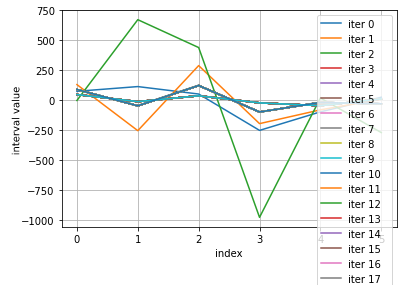
\includegraphics[width=12cm]{3.png}
    \label{fig:1s}
\end{figure}
 
    С помощью теоремы из пункта 2.1 получаем, что матрица является особенной.
    
    Субдифференциальный метод на данной системе не сходится за конечное число итераций.
    
    Для этой интервальной линейной системы алгоритм генерирует осциллирующую последовательность, которая, очевидно, не сходится ни к какому пределу. Интересно отметить, что правая часть этой системы шире, чем в предыдущем примере, а все элементы матрицы, кроме $a_{33}$, тоньше, что говрит о том, что данная ИСЛАУ еще лучше подчинаетсятеореме о сходимости. Тем не менее метод не работает.
  
  \subsection{Исследование}
    Сразу стоит отметить, что изменение параметра $\tau$ при применении метода к системам, на которых метод показывает хорошую сходимость, значительно замедляет работу.
    
    В качестве же эксперемента было принято решение внести изменения в компоненту $a_{33}$ и проверить сходимость метода. Был получен следующий результат:
\begin{table}[H]
			\centering
			\begin{tabular}{|c|c|c|c|}
				\hline
				$\textbf{a}_{33 - inf}$ & \textbf{Results} & $\textbf{a}_{33 - sup}$ & \textbf{Results}\\
				
				\hline
				$0.0$ & Расходимость & $-10.0$ & Сходимость \\
				
				\hline
				$0.5$ & Расходимость & $-9.5$ & Сходимость \\
				
				\hline
				$1.0$ & Расходимость & $-9.0$ & Сходимость \\
				
				\hline
				$1.5$ & Сходимость & $-8.5$ & Сходимость \\
				
				\hline
				$2.0$ & Расходимость & $-8.0$ & Сходимость \\
				
				\hline
				$2.5$ & Расходимость & $-7.5$ & Сходимость \\
				
				\hline
				$3.0$ & Расходимость & $-7.0$ & Сходимость \\
				
				\hline
				$3.5$ & Сходимость & $-6.5$ & Сходимость \\
				
				\hline
				$4.0$ & Расходимость & $-6.0$ & Сходимость \\
				
				\hline
				$4.5$ & Расходимость & $-5.5$ & Сходимость \\
				
				\hline
				$5.0$ & Сходимость & $-5.0$ & Сходимость\\
				
				\hline
				$5.5$ & Сходимость & $-4.5$ & Сходимость\\
				
				\hline
				$6.0$ & Расходимость & $-4.0$ & Сходимость \\
				
				\hline
				$6.5$ & Расходимость & $-3.5$ & Сходимость \\
				
				\hline
				$7.0$ & Сходимость & $-3.0$ & Сходимость \\
				
				\hline
				$7.5$ & Расходимость & $-2.5$ & Сходимость \\
				
				\hline
				$8.0$ & Сходимость & $-2.0$ & Сходимость \\
				
				\hline
				$8.5$ & Сходимость & $-1.5$ & Сходимость \\
				
				\hline
				$9.0$ & Сходимость & $-1.0$ & Сходимость \\
				
				\hline
				$9.5$ & Сходимость & $-0.5$ & Расходимость \\

				\hline
				
			\end{tabular}
			\caption{Результаты коррекции значения интервала $a_{33}$ при $\tau=1$}
		\end{table}
		
c каждым шагом изменялось значение $inf$ или $sup$ интервала $a_{33}$.
Несложно заметить, что второе действие принесло более однозначный результат.

Проведем еще один эксперимент и попробуем изменить параметр релаксации на $\tau=0.6$, продолжая варьировать значение $inf$ и $sup$

\begin{table}[H]
			\centering
			\begin{tabular}{|c|c|c|c|}
				\hline
				$\textbf{a}_{33 - inf}$ & \textbf{Results} & $\textbf{a}_{33 - sup}$ & \textbf{Results}\\
				
				\hline
				$0.0$ & Расходимость & $-10.0$ & Сходимость \\
				
				\hline
				$0.5$ & Расходимость & $-9.5$ & Сходимость \\
				
				\hline
				$1.0$ & Расходимость & $-9.0$ & Сходимость \\
				
				\hline
				$1.5$ & Сходимость & $-8.5$ & Сходимость \\
				
				\hline
				$2.0$ & Сходимость & $-8.0$ & Сходимость \\
				
				\hline
				$2.5$ & Сходимость & $-7.5$ & Сходимость \\
				
				\hline
				$3.0$ & Сходимость & $-7.0$ & Сходимость \\
				
				\hline
				$3.5$ & Сходимость & $-6.5$ & Сходимость \\
				
				\hline
				$4.0$ & Сходимость & $-6.0$ & Сходимость \\
				
				\hline
				$4.5$ & Сходимость & $-5.5$ & Сходимость \\
				
				\hline
				$5.0$ & Сходимость & $-5.0$ & Сходимость\\
				
				\hline
				$5.5$ & Сходимость & $-4.5$ & Сходимость\\
				
				\hline
				$6.0$ & Сходимость & $-4.0$ & Сходимость \\
				
				\hline
				$6.5$ & Сходимость & $-3.5$ & Сходимость \\
				
				\hline
				$7.0$ & Сходимость & $-3.0$ & Сходимость \\
				
				\hline
				$7.5$ & Сходимость & $-2.5$ & Сходимость \\
				
				\hline
				$8.0$ & Сходимость & $-2.0$ & Сходимость \\
				
				\hline
				$8.5$ & Сходимость & $-1.5$ & Сходимость \\
				
				\hline
				$9.0$ & Сходимость & $-1.0$ & Сходимость \\
				
				\hline
				$9.5$ & Сходимость & $-0.5$ & Расходимость \\

				\hline
				
			\end{tabular}
			\caption{Результаты коррекции значения $a_{33}$ при $\tau=0.6$}
		\end{table}  $\Longrightarrow$ область сходимости расширилась

\end{document}